\documentclass[titlepage]{article}
\usepackage[utf8]{inputenc}
\usepackage{amsthm}
\usepackage{mathtools}
\usepackage{graphicx} %obsluga grafiki
\usepackage{epstopdf} %obsluga eps
%\usepackage[nottoc, notlof, numbib]{tocbibind} % wyswietlenie bibliografii w spisie tresci
\usepackage{url}
\usepackage{cite}
\usepackage[justification=centering]{caption}
\usepackage{float}
\newcommand{\multifigcaption}{\captionsetup{justification=justified}}

\usepackage{enumitem}
\usepackage{url}
\usepackage[colorlinks=false]{hyperref}
\usepackage{microtype}
\usepackage{array}
\usepackage[table]{xcolor}


\title{Research Skills and Methodologies\\Path Optimization of 3D Printer}
\author{Michał Kowalski, 195447\\Piotr Lechowicz, 195651}
\date{}

\begin{document}
\maketitle

\tableofcontents
\newpage

\section{Introduction}
Nowadays 3D printing is one of the fastest developing technologies. It allows us to convert digital 3D models into solid 3 dimensional objects. It is commonly used in prototyping because it allows to make 3D object without a need to use forms. The main advantages of 3D printing technology are: low cost of the printer, low cost of printing object, variety of materials and variety of technologies.
To use this technology, we need to:
\begin{enumerate}
\item create a 3D model of our object,
\item "cut" (convert) it into set of very thin layers,
\item choose path for printing tool.
\end{enumerate}
Our path should consist of points from layer currently being printed. Tool have to visit each point exactly once and can move without printing. Task is to minimize "cost" of moving between all succeding points in our path. We can calculate it for each pair in (at least) three ways:
\begin{enumerate}
\item distance between points,
\item time needed for move from one to next,
\item energy needed for that move.
\end{enumerate}
We are assuming that our printing tool is a point moving on two perpendicular axes.

Another task was to write an environment, which will deliver layers for algorithms, provide methods commonly used in finding path, and will save and show results in human-friendly way, including graphical representation of found path. It should also be open to addition of new algorithms.

\pagebreak

\section{Mathematic description of problem}
Given:
\begin{itemize}
\item printing layer as an array (size n x m) of binary points, where
\begin{equation}
\label{layer}
X_{i,j}=\left\{ \begin{array}{rl}
 1 &\mbox{if printing point} \\
 0 &\mbox{otherwise}
       \end{array} \right. \mbox{and} i \in n, j \in m
\end{equation}
\item cost for move between two points calculated in one of three possible ways:
\begin{itemize}
\item minimum distance
\begin{equation}
\label{distance_cost}
L_{P_{a,b}, P_{c,d}} = \sqrt{(a-c)^2+(b-d)^2}
\end{equation}
\item minimum time (only axis which need to move more)
\begin{equation}
\label{time_cost}
L_{P_{a,b}, P_{c,d}} = max(|a-c|, |b-d|)
\end{equation}
\item minimum energy (sum of movements, due to separate engines)
\begin{equation}
\label{energy_cost}
L_{P_{a,b}, P_{c,d}} = |a-c|+|b-d|
\end{equation}
\end{itemize}
where $a, c \in n$ and $b, d \in m$.
\end{itemize}

Find:
\begin{itemize}
\item order of visiting points $V=[X_1, X_2, ..., X_p]$ where \textit{p} is count of points in layer,
\item total cost of path consisting of visiting points $L=\sum\limits_{k=2}^p (L_{X_{k-1}, X_k})$,
\item time of calculations for each considered algorithm,
\end{itemize}
such that length of path and time of calculations are minimized.

\pagebreak
\section{Description of Algorithms}
Following algorithm were implemented:
\begin{itemize}
\item Left-To-Right algorithm
\item Snake algorithm
\item Edge Following algorithm
\item Greedy algorithm
\item Two Opt algorithm
\item Greedy Two Opt algorithm
\item Harmony Search algorithm
\item Greedy Harmony algorithm
\item Simulated Annealing algorithm
\item Greedy Annealing algorithm

\end{itemize}
All implementations of algorithms are based on superclass, which makes all necessary communication between environment and algorithm, like:
\begin{itemize}
\item setting up an algorithm, e.g. getting a layer to print,
\item sending results of algorithm to rest of application,
\item measuring time of calculations.
\end{itemize}
Therefore, algorithms only have to do all calculations in method returning a path, and optionally set up all variables in separate method. It also simplifies adding new algorithms, because all they have to do is implement this method, and they have to be added to list of algorithms.

\subsection{Left-To-Right algorithm}
This algorithm was created mostly for testing purposes. It had to be as simple as possible, and still find correct route, so it allows to test how environment works with algorithms in general.

Algorithm starts in top-left corner and goes line-by-line from left to right, adding to route all points on its way. And because only point to print are on found route, printer will go straight from last point in one line, to first in next one containing any points. Behaviour of this algorithm is similar to traditional paper printes.

\subsection{Snake algorithm}
This algorithm is an improvement of Left-To-Right algorithm. Instead of going always from left to right, it finds a closer end of next line containing points, and then goes to another end of it. Differences between them are show on figure \ref{img:ltr-vs-snake}.

\begin{figure}
\begin{center}
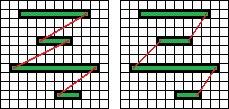
\includegraphics[scale=2]{img/ltr-vs-snake}
\caption{Left-To-Right algorithm on the left, Snake algorithm on the right}
\label{img:ltr-vs-snake}
\end{center}
\end{figure}

\subsection{Edge Following algorithm}
This algorithm tries to start from edge of a shape on a layer, and tries to get to the middle of it, and later choose next shape.
It's made in few steps:
\begin{enumerate}
\item Check, if there's any points left.
\item Find all edges on layer.
\item Go to closest point belonging to found edges.
\item As long, as there is any neighbour of current point, go to it.
\item Go back to 1.
\end{enumerate}
Finding edges and neighbours depend on chosen cost function. For example, diagonal neighbours exists only for time cost type.

%------------------------------------subsection greedy----------------------------------------------------------------------------

\subsection{Greedy algorithm}

A greedy algorithm is an algorithm which always makes the choice that looks best at the moment. It makes a locally optimal choice with the hope of finding a global optimum. Greedy algorithms do not always yield optimal solution nevertheless they may give solution that approximates a global optimal solution in a reasonable time. Commonly greedy strategy for the travelling salesman problem is as follows: at each stage visit an unvisited point nearest to the current city. In case of this particular problem of path finding in 3D printer, locally optimal solution was slightly modified. It has to be well described because of its good results it was used to construct further hybrid algorithms.

\subsubsection{Greedy adjacent points modification}

Lets consider an example where locally optimal solution is based only on distance between two points. In all examples distance between two adjacent points equals to one. Figure \ref{img:greedy/example-points-on-layer} shows example layer with few points. If optimal choice is made only by considering distance, the path would look as it is shown in the figure \ref{img:greedy/example-path-sol-1}.

\begin{figure}[H]
	\begin{center}
		\begin{minipage}{.45\linewidth}
			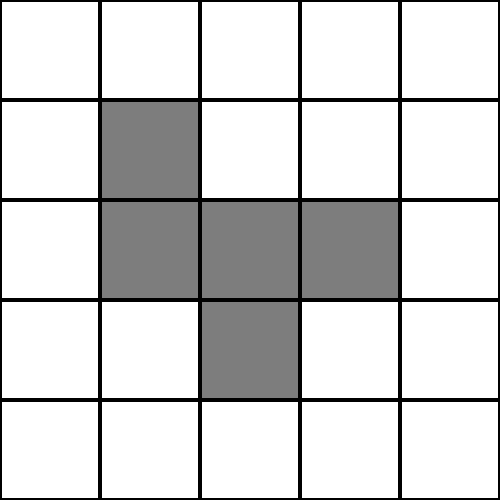
\includegraphics[width=\textwidth]{img/greedy/example-points-on-layer.png}
			\multifigcaption
			\caption{Example points on layer \newline}
			\label{img:greedy/example-points-on-layer}
		\end{minipage}
		\hspace{.05\linewidth}
		\begin{minipage}{.45\linewidth}
			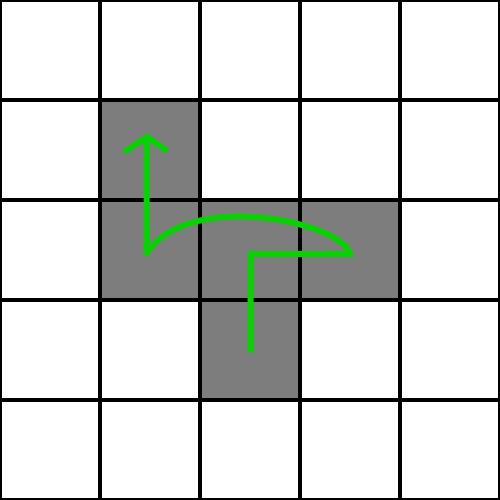
\includegraphics[width=\textwidth]{img/greedy/example-path-sol-1}
			\multifigcaption
			\caption{Path number 1 for example layer}
			\label{img:greedy/example-path-sol-1}
		\end{minipage}
	\end{center}
\end{figure}

\begin{gather*}
	L_1 = 5 \mbox{ ,} \\
	\mbox{where }L_1 \mbox{ is length of the path in the figure \ref{img:greedy/example-path-sol-1}}
\end{gather*}



On the other hand if we begin to consider locally optimal solution not only based on distance between source and target points but also on number of adjacent points to target point, we can notice that in some cases it is better to choose point a little further but with lower number of adjacent points. It is illustrated in the figure \ref{img:greedy/example-path-sol-2}.

\begin{figure}[H]
	\begin{center}
		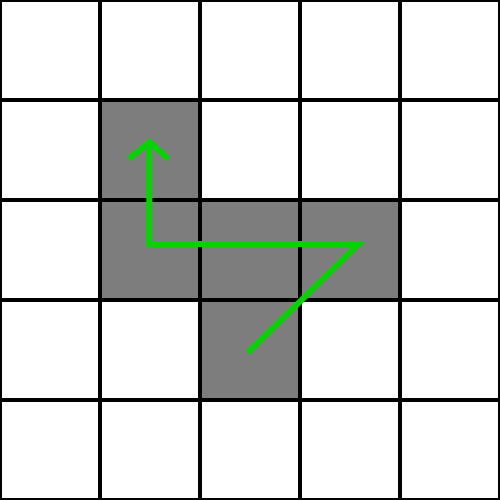
\includegraphics[width=0.5\textwidth]{img/greedy/example-path-sol-2}
		\caption{Path number 2 for example layer}
		\label{img:greedy/example-path-sol-2}
	\end{center}
\end{figure}

\begin{gather*}
	L_2 = 3 + \sqrt{2} \approx 4.41 \mbox{ ,} \\
	\mbox{where }L_2 \mbox{ is length of the path in the figure \ref{img:greedy/example-path-sol-2}}
\end{gather*}

Comparing distances from figure \ref{img:greedy/example-path-sol-1} and \ref{img:greedy/example-path-sol-2}  we can notice that point which is further but has only one adjacent point is a better choice than point which is closer but has two adjacent points. That's why in algorithm was introduced parameters describing how much algorithm will prefer points which are further but has lower number of adjacent points. 

 In all tests were used assumption that if distances are similar, it is each one of them isn't greater than the other one more than $0.42$ (it comes from subtraction of distances of these two paths on figures \ref{img:greedy/example-path-sol-1} and \ref{img:greedy/example-path-sol-2}), the best choice is to visit point which has the lowest number of adjacent points. If there is a point which has no adjacent point, it is the optimal choice. This way of proceeding helps to eliminate isolated points, which may finally determine result to be unsatisfying. Justification of this way of thinking is presented in figures \ref{img:greedy/example-path2-sol-1} and \ref{img:greedy/example-path2-sol-2}.
 
 \begin{figure}[H]
 	\begin{center}
 		\begin{minipage}{.45\linewidth}
 			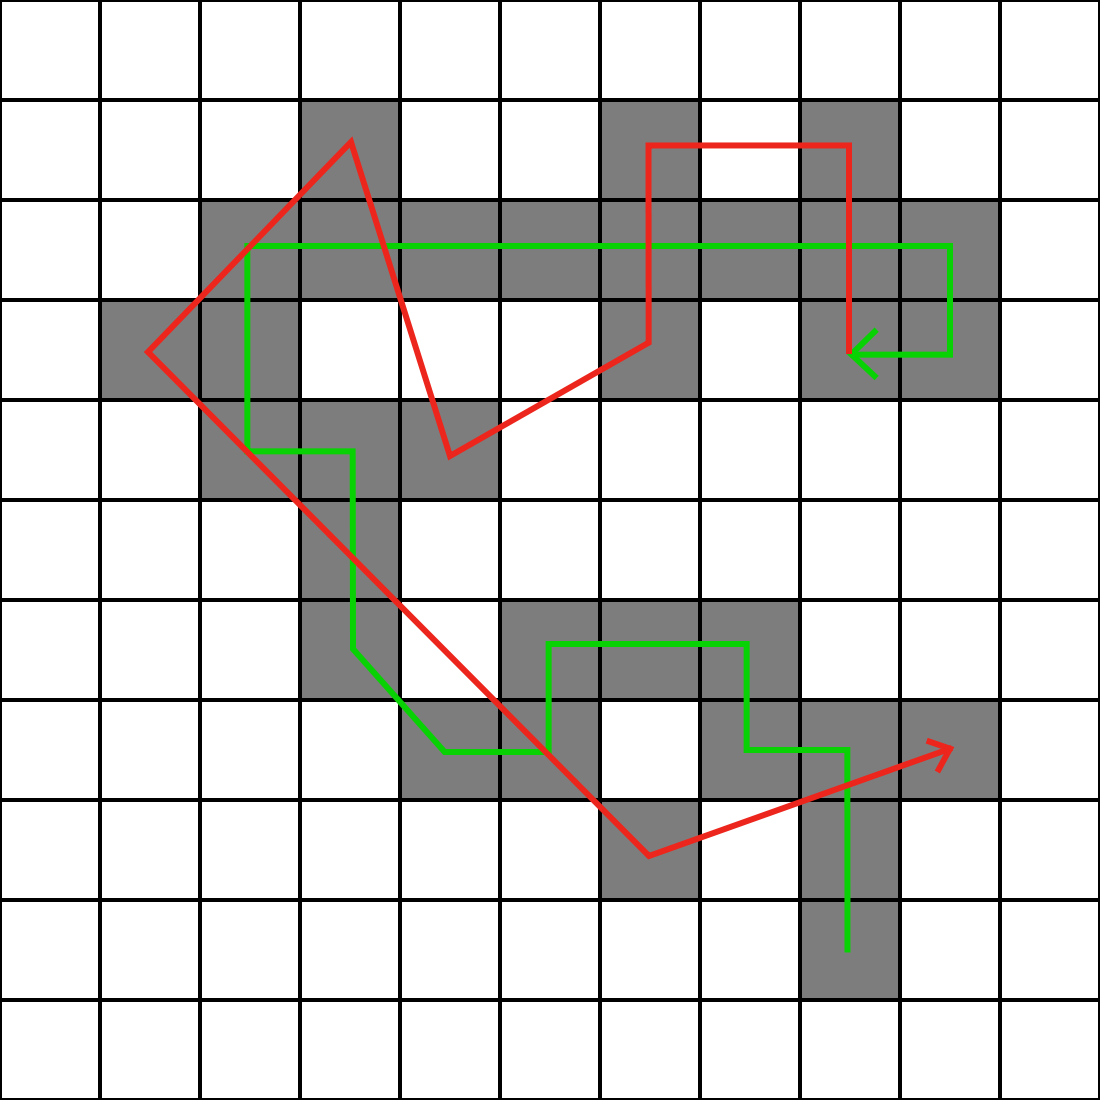
\includegraphics[width=\textwidth]{img/greedy/example-path2-sol-1.png}
			\multifigcaption
 			\caption{Path computed without considering number of adjacent points (the red one is an inefficient part of path)}
 			\label{img:greedy/example-path2-sol-1}
 		\end{minipage}
 		\hspace{.05\linewidth}
 		\begin{minipage}{.45\linewidth}
 			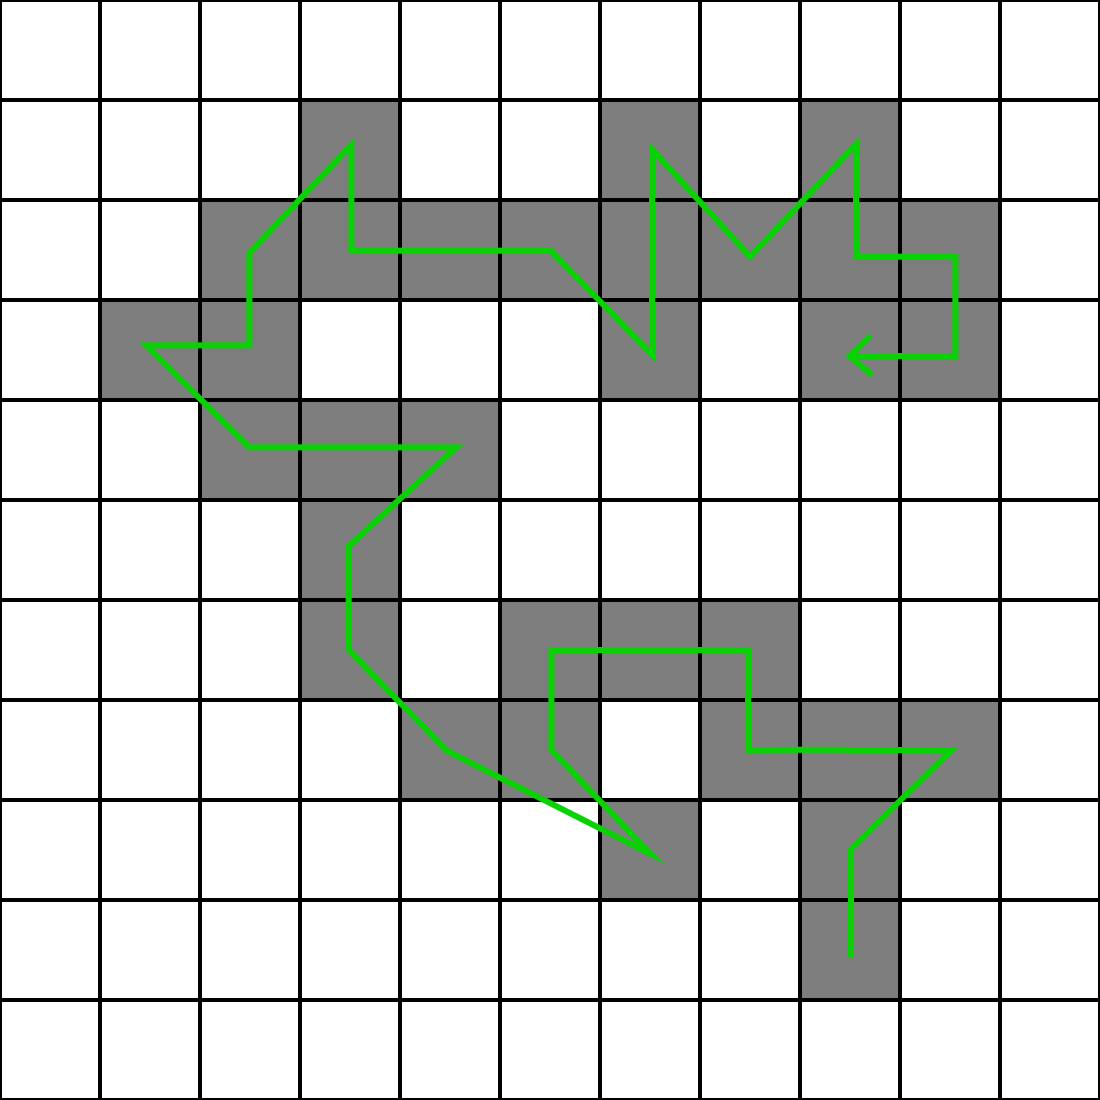
\includegraphics[width=\textwidth]{img/greedy/example-path2-sol-2.png}
			\multifigcaption
 			\caption{Path computed with considering number of adjacent points \newline \vspace{4mm}}
 			\label{img:greedy/example-path2-sol-2}

 		\end{minipage}
 	\end{center}
 \end{figure}
 
 In the figure \ref{img:greedy/example-path2-sol-1} total length of path is $L \approx 47.87$ and in the figure \ref{img:greedy/example-path2-sol-2} is $L \approx 35.96$. As we can see with the greater number of points to print the importance of not leaving isolated ones increases.
 
\subsubsection{Greedy neighbour searching modification}
 
 Another introduced improvement in the algorithm is the modification of process of searching the nearest unvisited point from the currently visited one. Most of the printing layers have rather densely distributed points, e. g. most of them are located in the centre of the layer. In order to reduce time needed for checking distances to all possible point to find the nearest one, algorithm firstly search the neighbourhood of currently visited point, it is places for possible points, which are not further than one unit in each side. In case of negative result algorithm extends searches to two units in each side. If in that process any point was obtained, algorithm starts looking for next move by searching a list of all possible points. Figures from \ref{img:greedy/example-neighbours-stating} to \ref{img:greedy/example-neighbours-neigh-solv} illustrate this part of algorithm.
 
\begin{figure}[H]
 	\begin{center}
 		\begin{minipage}{0.45\linewidth}
 			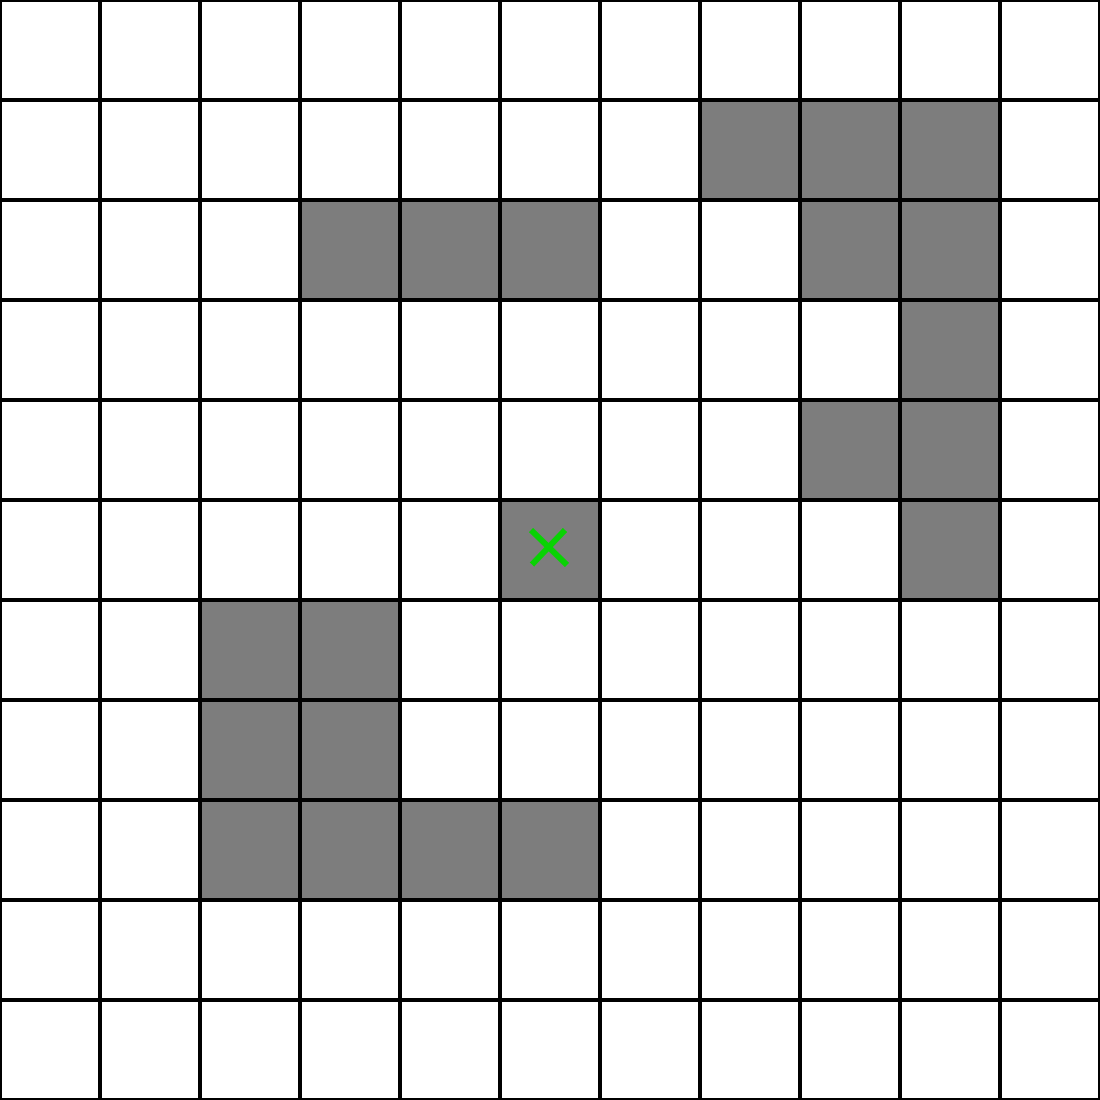
\includegraphics[width=\textwidth]{img/greedy/example-neighbours-starting.png}
 			\multifigcaption
 			\caption{Starting position for searching neighbourhood (green cross represent currently printed point)}
 			\label{img:greedy/example-neighbours-stating}
 		\end{minipage}
 		\hspace{.05\linewidth}
 		\begin{minipage}{.45\linewidth}
 			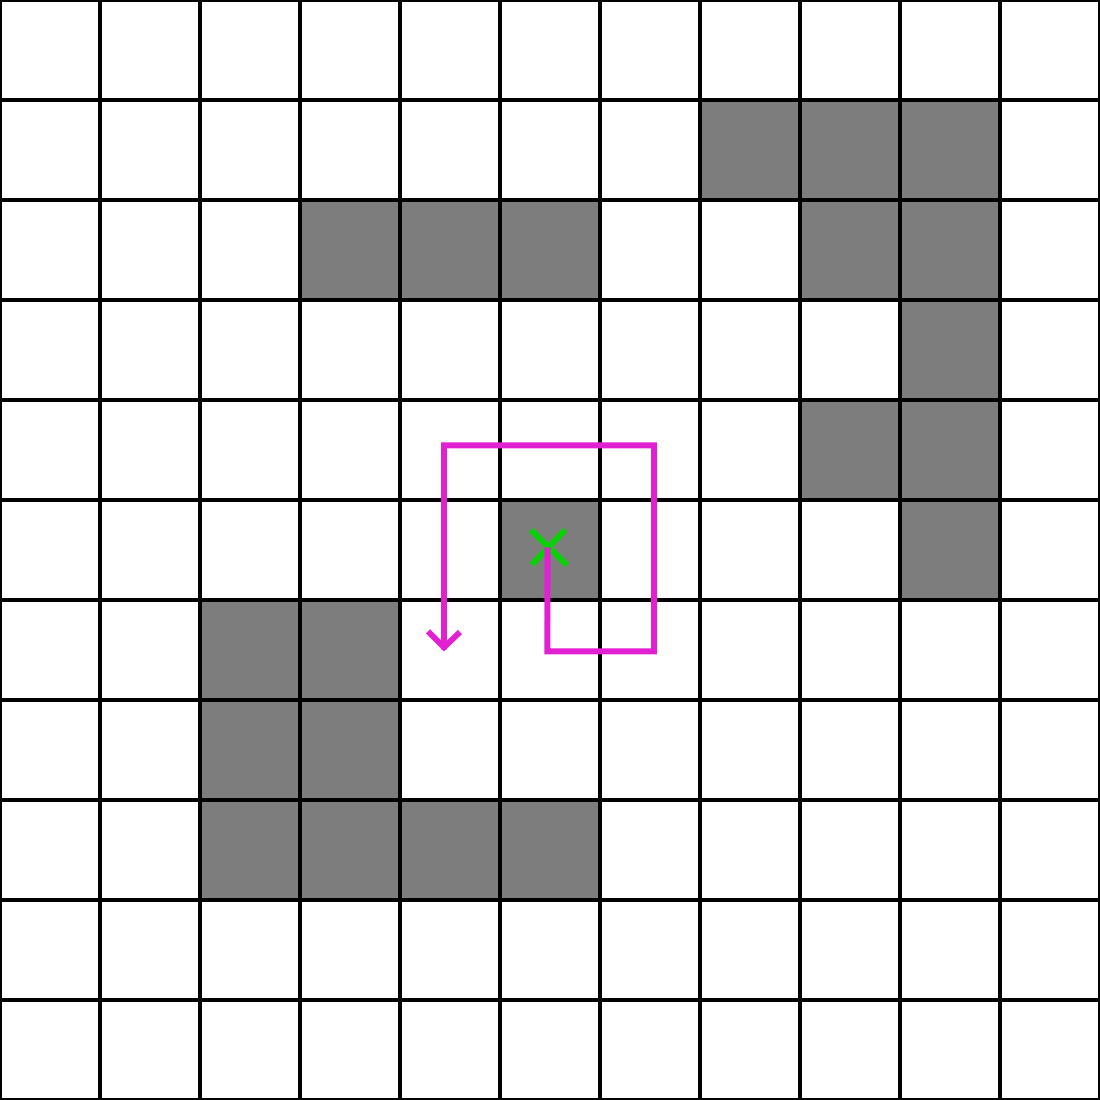
\includegraphics[width=\textwidth]{img/greedy/example-neighbours-neigh-1.png}
 			\multifigcaption
 			\caption{First iteration of searching \newline \vspace{4mm}}
 			\label{img:greedy/example-neighbours-neigh-1} 
 		\end{minipage}
	\end{center}
\end{figure}

In the figure \ref{img:greedy/example-neighbours-stating} we have starting point which was the latest one visited. Algorithm starts to search neighbourhood of the point. In the figure \ref{img:greedy/example-neighbours-neigh-1} is shown first iteration. Because algorithm didn't find any point it extends searches which is presented in the figure \ref{img:greedy/example-neighbours-neigh-2}. Because there are three possible solutions for the next move, algorithm has to chose the most optimal one. It considers both criteria - distance and number of adjacent points. The result is the upper one (figure \ref{img:greedy/example-neighbours-neigh-solv}).

\begin{figure}[H]
 	\begin{center}
 		\begin{minipage}{0.45\linewidth}
 			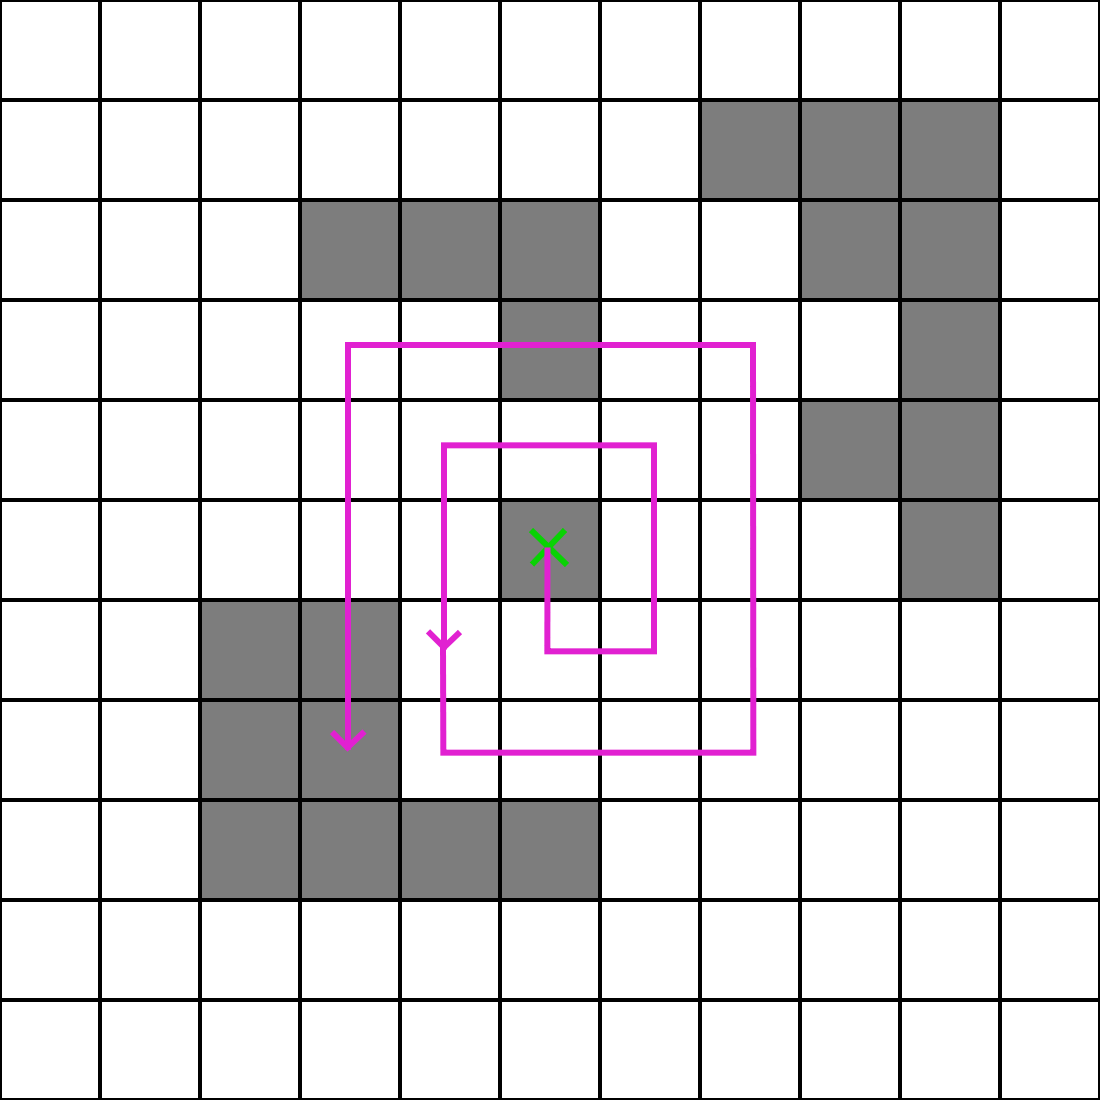
\includegraphics[width=\textwidth]{img/greedy/example-neighbours-neigh-2.png}
 			\multifigcaption
 			\caption{Second iteration of searching}
 			\label{img:greedy/example-neighbours-neigh-2}
 		\end{minipage}
 		\hspace{.05\linewidth}
 		\begin{minipage}{.45\linewidth}
 			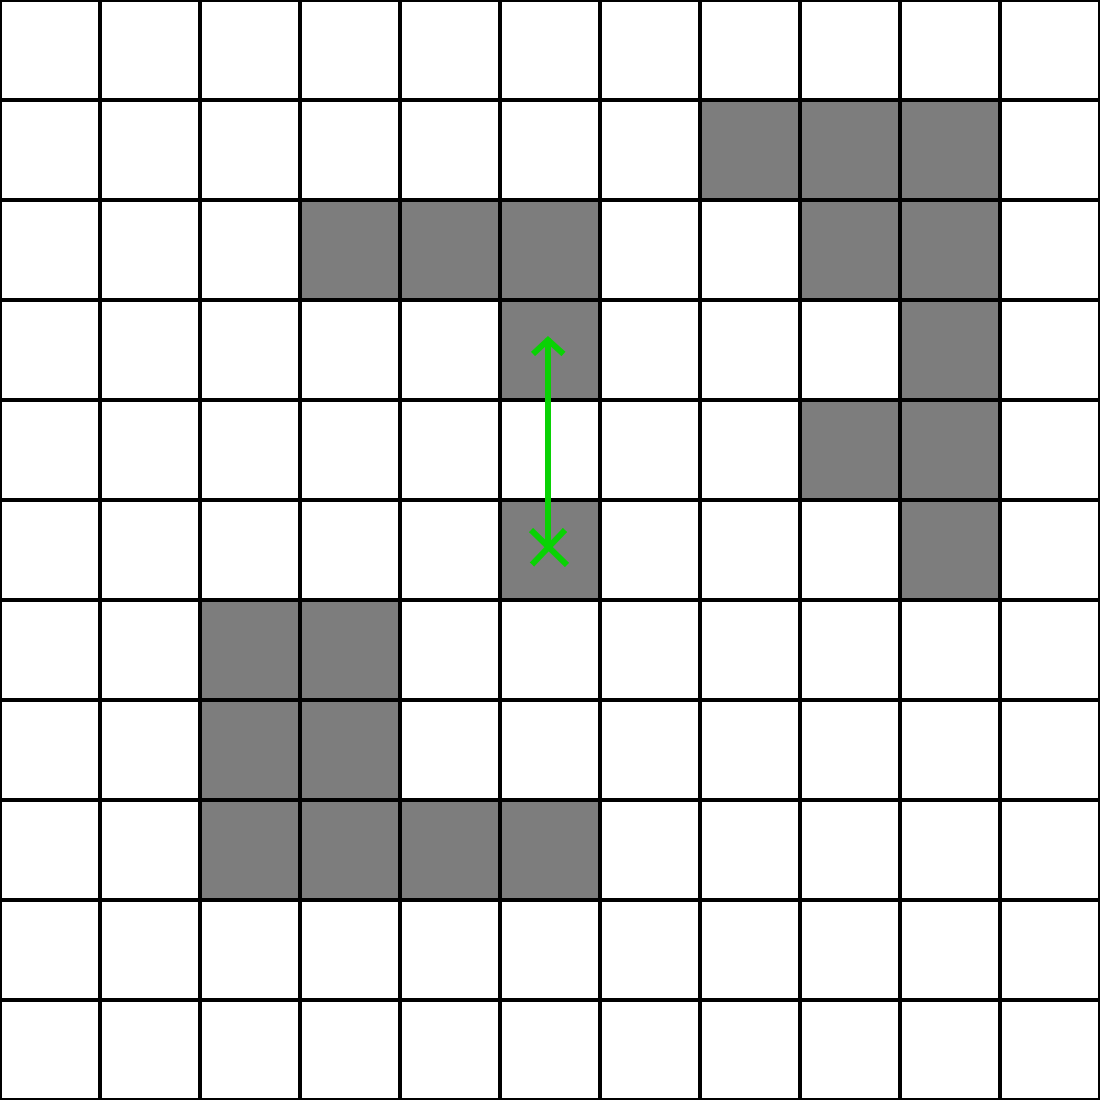
\includegraphics[width=\textwidth]{img/greedy/example-neighbours-neigh-solv.png}
 			\multifigcaption
 			\caption{Move of the printing tool \newline}
			\label{img:greedy/example-neighbours-neigh-solv} 
		\end{minipage}
	\end{center}
\end{figure}

\subsubsection{Greedy parameters}

Implemented greedy algorithm allows parametrization in order to adapt it to different kinds of layers. The list of parameters with its description:

\begin{itemize}
	\item \texttt{seed} - seed of the random. Some parts of algorithm are randomized. Instance of Java class \texttt{Random} is used to generate a stream of pseudorandom numbers. It uses a 48-bit seed as the initial value of the internal state of pseudorandom number generator. If parameter is set to $-1$ the seed is the current time in miliseconds since January 1, 1970.
	
	\item \texttt{nrOfThreads} - number of threads. Algorithm can consider different points as a starting point. Number of threads determine the amount of concurrently finding solutions.
	
	\item \texttt{nrOfNeighboursForStartingPoint} - number of neighbours for starting point. Preferable amount of adjacent points for the starting one. If there are no more such points, remaining starting points are generated randomly.
	
	\item \texttt{nrOfPointsNeededToCheckArray} - number of points needed to check array. Normally algorithm searches neighbourhood for finding nearest point. When number of remaining points to print is lower than this parameter algorithm straight away starts checking all possible points for finding the nearest one, without considering neighbourhood of the point.
	
	\item \texttt{bestNrOfNeighours} - best number of neighbours. Sets preferable number of adjacent points for the next moves of printing tool.
	
	\item \texttt{weightOfNeighbours} - weight of neighbours. It determines how much algorithm would prefer points which are further but have closer number of adjacent points to the parameter \texttt{bestNrOfNeighbours}. It is simply acceptable difference of distances between this point and the nearest one.
	
	\item \texttt{weightOfDistance} - weight of distances. It determines how much algorithm would prefer points which are nearer but their number of adjacent points is greater than defined in parameter \texttt{bestNrOfNeighbours}. It is simply acceptable difference of distances between the nearest point and the point with closer number of neighbours to the preferable one.
	
\end{itemize}

\subsubsection{Greedy procedure}

The overall procedure of finding path realized by this algorithm:

\begin{enumerate}
	\item create and fill table of neighbours - the table which contains amount of adjacent points for each of them
	\item set starting point for each thread
	\item start threads:
	\begin{enumerate}[label*=\arabic*.]
		\item if there are more unvisited points than \texttt{nrOfPointsNeededToCheckArray}:
		\begin{enumerate}[label*=\arabic*.]
			\item search for the nearest point in the neighbourhood
			\item if point wasn't found search for optimal point in the list of all remaining points.
		\end{enumerate}
		\item otherwise:
		\begin{enumerate}[label*=\arabic*.]
			\item search for optimal point in the list of all remaining points
		\end{enumerate}
	\end{enumerate}
	\item after joining threads get all result paths from them
	\item return path with lowest distance
\end{enumerate}

Procedure of finding optimal point ($d[point]$ is the distance from current point to that point, $n[point]$ is the number of adjacent points):

\begin{enumerate}
	\item take distance and number of adjacent points from first point as a best ones ($best \leftarrow point$)
	\item if $d[best] \leq 1 + \mbox{\texttt{weightOfNeighbours}}$ and $n[best] \leq \mbox{\texttt{bestNrOfNeighbours}}$, return this point as an optimal (\texttt{return} $best$)
	\item while there are unchecked points:
	
	\begin{enumerate}[label*=\arabic*.]
		\item if $d[next] < d[best] - \mbox{\texttt{weightOfDistance}}$ take this point as a best one ($best \leftarrow next$)
		\item else if $d[next] < d[best] + \mbox{\texttt{weightOfNeighbours}}$ and $n[next] < n[best]$ take this point as a best one ($best \leftarrow next$)
		\item if $d[best] \leq 1 + \mbox{\texttt{weightOfNeighbours}}$ and $n[best] \leq \mbox{\texttt{bestNrOfNeighbours}}$ return this point as an optimal one (\texttt{return} $best$)
		\item else continue while loop
	\end{enumerate}
\end{enumerate}

%--------------------------------------------------------subsection----------------------------------------------------------------

\subsection{Two Opt algorithm}

This algorithm is based on the exchange or swap of a pair of edges. To swap two edges $(a, b)$ and $(c, d)$, the nodes of the pair of edges are rearranged as $(a, c)$ and $(b, d)$. The algorithm tries to untangle crossing edges. There were implemented two variety of this algorithm. In the first one it searches for first swap which will result in shortest total length of path and executes it. The procedure is repeated till no improvements are found. The difference between the second one and the first one is that it searches at each iteration for the best possible swap and then executes it. The idea of the algorithm is presented in the figures \ref{img:twoopt/path1} and \ref{img:twoopt/path2}.

\begin{figure}[H]
	\begin{center}
		\begin{minipage}{.45\linewidth}
			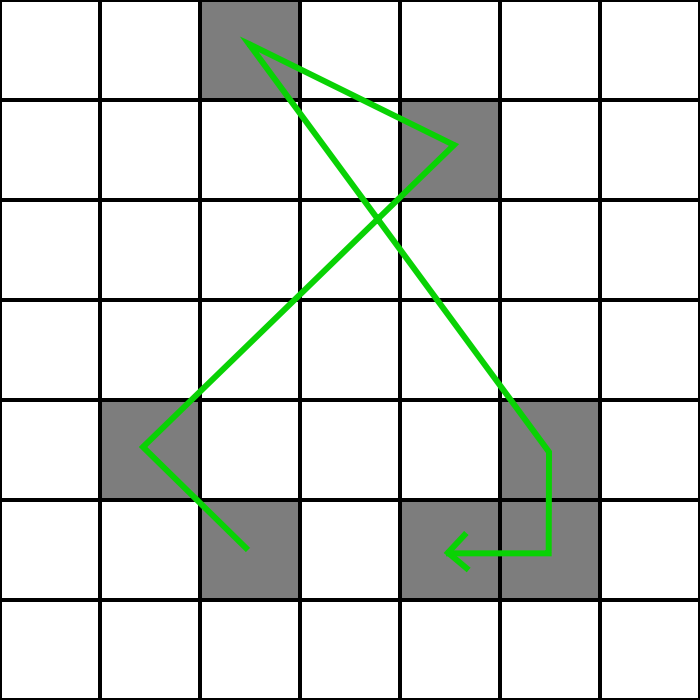
\includegraphics[width=\textwidth]{img/twoopt/path1.png}
			\multifigcaption
			\caption{Path before swapping edges}
			\label{img:twoopt/path1}
		\end{minipage}
		\hspace{.05\linewidth}
		\begin{minipage}{.45\linewidth}
			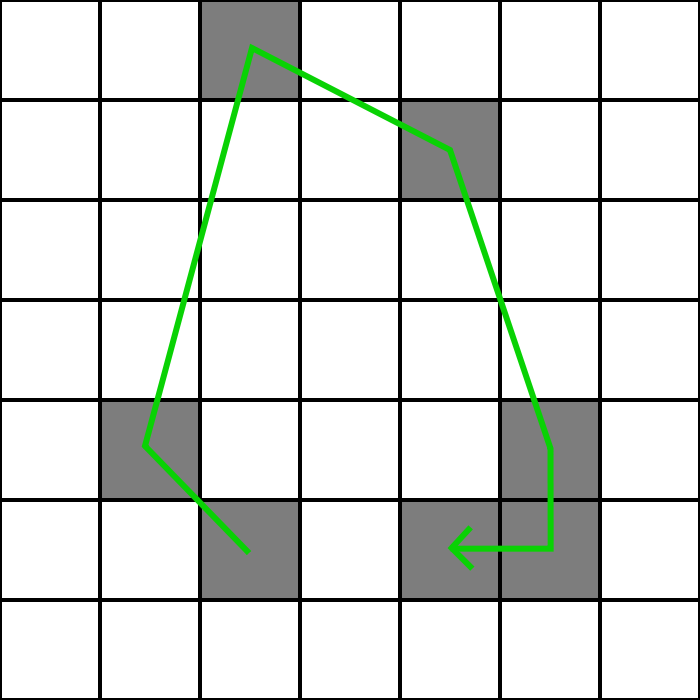
\includegraphics[width=\textwidth]{img/twoopt/path2.png}
			\multifigcaption
			\caption{Path after swapping edges}
			\label{img:twoopt/path2}
			
		\end{minipage}
	\end{center}
\end{figure}

\subsubsection{Two Opt parameters}

\begin{itemize}
	\item \texttt{isGreedy} - is greedy flag. When \texttt{isGreedy} is \texttt{false} algorithm searches for the best possible swap, it is it checks all possible pairs of edges and chooses the most profitable. If flag is \texttt{true} it executes swap with first found pair of edges which will shorten the total length of path.
	
	\item \texttt{maxNrOfIterations} - maximal number of iterations. If it is set to $-1$ algorithm improves path till it cannot find any more beneficial swaps. If it is greater than $0$, algorithm makes exact number of swaps.	
\end{itemize}

\subsubsection{Two Opt procedure}

\begin{enumerate}
	\item find first random path
	\item if \texttt{isGreedy} $==$ \texttt{true}: \\
	\hspace*{5mm} find first beneficial pair of edges \\
	else:\\
	\hspace*{5mm} find the most profitable pair of edges
	\item if wasn't find such a pair return from algorithm
	\item otherwise swap edges
	\item if maximal number of iterations is not defined or is defined but $\mbox{\texttt{currentIteration}} < \mbox{\texttt{maxNrOfIterations}}$ jump to 2nd step
	\item else return from algorithm
\end{enumerate}

%------------------------------------------------------subsection--------------------------------------------

\subsection{Greedy Two Opt algorithm}

Greedy Two Opt is composed of two algorithms. The first stage is to find path through Greedy algorithm. This path is passed as an initial path to Two Opt algorithm. The idea behind it is that it is much better to improve path close to the optimal solution than totally randomly selected. It takes much less iterations for Two Opt to finds path which it cannot improve any more. 

\subsection{Harmony Search algorithm}

The Harmony Search is an algorithm inspired by the improvisation process of Jazz musicians. If musician plays he can choose to select a sound from his memory or randomly select other note. If it 'sounded' good he can 'try' to remember it for future use. The memory is a list of travelling salesman problem solutions (they must start from the same point). Algorithm find new solution with the following way: it starts from the first point and with certain probability chooses next point from memory or chooses from rest of the available points. It is repeated till all points are used exactly once. If it is generated new solution it is compared to the solutions within the memory. If found solution is better than the worst from the memory, the one from the memory is removed, and this one is added. This steps are repeated for particular number of iterations (time of jazz improvisation). Because of its high randomness of beginning paths added to memory, it is used as a part of a hybrid algorithm.

\subsubsection{Harmony Search parameters}

\begin{itemize}
	\item \texttt{seed} - seed of the random. Similarly to the Greedy algorithm's seed.
	
	\item \texttt{memorySize} - size of the memory. Amount of best paths being stored in the memory.
	
	\item \texttt{nrOfIterations} - number of iterations. How many times algorithm repeats finding path and comparing if it is better than paths in the memory.
	
	\item \texttt{memoryProbability} - probability that algorithm chooses point from the memory rather than randomly from the rest of unvisited points.
\end{itemize}

\subsubsection{Harmony Search procedure}

\begin{enumerate}
	\item choose starting point
	\item fill memory with random paths, each starts from the starting point
	\item create a $new path$ containing only starting point
	\item if next point is taken from memory:
	\begin{enumerate}[label*=\arabic*.]
		\item randomly select one of the paths within the memory
		\item take point with the corresponding place, it is, if is searched $n-th$ point for the $new path$ it is taken $n-th$ point from path from the memory
		\item if that point is already in $new path$, the point is exchange with the one being chosen randomly from the rest of unvisited points in this iteration
		\item add point to the $new path$
		\item if $new path$ is not containing all points from the layer, algorithm jumps to 4th step
	\end{enumerate}
	else
	\begin{enumerate}[label*=\arabic*.]
		\item randomly select point from the list of unvisited points in this iteration and add it to $new path$
		\item if $new path$ is not containing all points from the layer, algorithm jumps to 4th step
	\end{enumerate}
	\item if $new path$ is better than the worst one in the memory, they are swap, otherwise this new solution is rejected
	\item steps from 3 to 5 are repeated \texttt{nrOfIterations} times
	\item return best path from the memory
	
\end{enumerate}

\subsection{Greedy Harmony algorithm}

The first stage of this algorithm is to find solution with Greedy algorithm and then it is passed as an initial solution to Harmony Search. The same solution is added to the harmony's memory as many times as it is necessary. Then Harmony Search algorithm tries to find solution closer to optimal. Because of the highly randomness of Harmony Search, setting starting path as already close to optimal solution may highly improves results of an algorithm.

\subsection{Simulated Annealing algorithm}

Simulated Annealing algorithm is inspired by annealing process in metallurgy. It emulates the physical process in which solid is firstly heated and then slowly cooled. With higher temperature metal is more vulnerable to deformation because of providing energy needed to break bonds. While the temperature becomes lower and lower it is harder to deform metal. In case of Simulated Annealing algorithm the temperature determines the probability of taken worse solution than currently obtained one in the future consideration. With lower temperature algorithm less likely takes worse solution. During whole process the best found solution is kept in memory, and replaced if better one is obtained. New solutions are found by swapping two randomly chosen edges. When temperature reaches earlier define minimum, algorithm stops. The probability of acceptance worse solution is calculated as follows:

\[e^{-\frac{J(j)-J(i)}{T(t)}}\mbox{,}\]
	where $J(i)$ is total distance of currently found solution, $J(i)$ is total distance of the best found solution and $T(t)$ is the temperature of time where the new solution was obtained.


\subsubsection{Simulated Annealing parameters}

\begin{itemize}
	\item \texttt{seed} - seed of the random. Similarly to the Greedy algorithm's seed.
	
	\item \texttt{temperatureMin} - minimal temperature. Temperature at which algorithm stops.
	
	\item \texttt{coolingRate} - cooling rate. It determines how fast temperature is decreasing. New temperature is get by multiplying currently one by this factor.
	
	\item \texttt{iterationsOnTemperature} - how many iterations algorithm does on each temperature state, it is, how many times it tries to find better solution with the same probability of acceptance worse solution.
	
	\item \texttt{maxNrOfIterationsWithNoImprovement} - maximal number of algorithm's iterations without finding better path. It prevents from pointless execution of algorithm when it cant find better solution.
\end{itemize}

\subsubsection{Simulated Annealing procedure}

\begin{enumerate}
	\item obtain randomly first solution
	\item set this solution as the $best$ one and as a $currentpath$
	\item select randomly two edges and swap them ($newpath \leftarrow swap(currentpath)$)
	\item if $distance[newpath] < distance[currentpath]$:
	\begin{enumerate}[label*=\arabic*.]
		\item $currentpath \leftarrow newpath$
		\item if $distance[currentpath] < distance[best]$: \\
		\hspace*{5mm} $best \leftarrow currentpath$
	\end{enumerate}
	else:
	\begin{enumerate}[label*=\arabic*.]
		\item take $newpath$ as a $currentpath$ with calculated probability for this temperature
	\end{enumerate}
	\item repeat steps 3 to 4 \texttt{iterationsOnTemperature} times
	\item calculate new temperature ($temperature \leftarrow \mbox{\texttt{coolingRate}}*temperature)$)
	\item assign best path to current path ($currentpath \leftarrow best$)
	\item repeat steps 2 to 7 while $temperature > minimal\_temperature$ or algorithm doesn't find better solution for \texttt{maxNrOfIterationsWithNoImprovement} iterations
	\item return $best$ path
	
\end{enumerate}

\subsection{Greedy Annealing algorithm}

In this algorithm initial path for Simulated Annealing is obtained by executing Greedy algorithm. All procedure steps and parameters are the same as in both of these algorithms. Simulated Annealing may be much more efficient if it starts with solution not o far from the optimal one. 

\section{Experiments}

\subsection{Environment}
Test environment was implemented, to provide:
\begin{itemize}
\item delivering chosen layers to algorithms,
\item graphical representation of layer and path,
\item displaying and showing to file results of algorithms,
\item easy adding of new algorithms (by inheriting one class and adding it to algorithm's list),
\item methods for reading algorithm's parameters from file.
\end{itemize}

\subsection{Test layers}
Images used as test layers are in "img" directory added to this report.

\subsection{Methodology}

During tests with layers were taken following assumptions. If algorithms are tested on the same layer they should be running with the same parameters, e. g. if Greedy algorithm and Simulated Annealing algorithm were used to find path in the specific layer, the Greedy Annealing algorithm should run with parameters the same as in each of the partial algorithm. It allows to objectively decide whether there are advantages coming from hybrid algorithms.

\section{Results}
For very short calculations, measured time can has very big differences between one measurement and another one with the same algorithm/params.

All result images and text files are added to this report in "results" directory.

In tables ... ... are presented example results of comparison of algorithms three different layers.

Picture "sp-4.png" which is presented on the figure \ref{img:results/sp-4} has many points and each one has many adjacent point. In table \ref{tab:results-sp-4} are presented results. In figures \ref{img:results/sp-4-ef-time}, \ref{img:results/sp-4-greedy-two-opt} and \ref{img:results/sp-4-greedy-harmony} are shown example paths.

\begin{figure}[H]
	\begin{center}
		\begin{minipage}{.45\linewidth}
			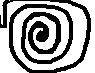
\includegraphics[width=\textwidth]{img/results/sp-4.png}
			\multifigcaption
			\caption{Layer sp-4 \newline}
			\label{img:results/sp-4}
		\end{minipage}
		\hspace{.05\linewidth}
		\begin{minipage}{.45\linewidth}
			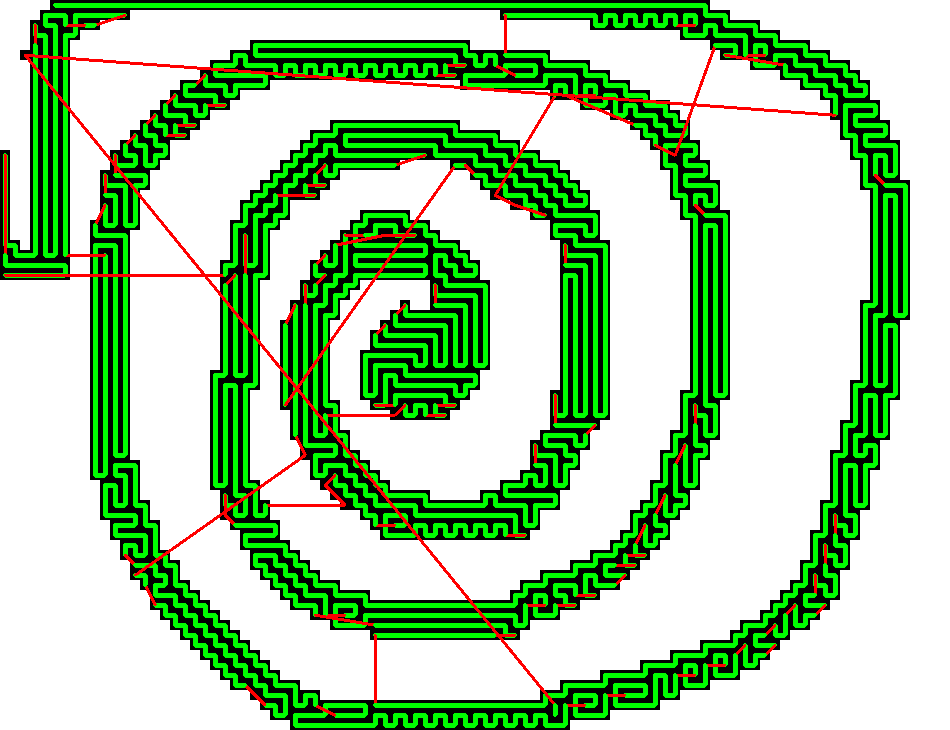
\includegraphics[width=\textwidth]{img/results/sp-4-ef-energy.png}
			\multifigcaption
			\caption{Edge Follower solution for layer sp-4}
			\label{img:results/sp-4-ef-energy}
		\end{minipage}
	\end{center}
\end{figure}

\begin{figure}[H]
	\begin{center}
		\begin{minipage}{.45\linewidth}
			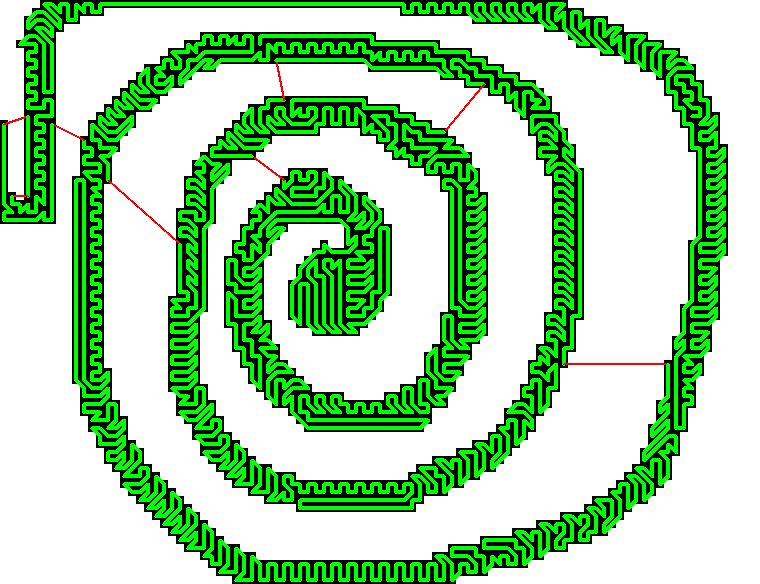
\includegraphics[width=\textwidth]{img/results/sp-4-greedy-two-opt.png}
			\multifigcaption
			\caption{Greedy Two Opt solution for layer sp-4}
			\label{img:results/sp-4-greedy-two-opt}
		\end{minipage}
		\hspace{.05\linewidth}
		\begin{minipage}{.45\linewidth}
			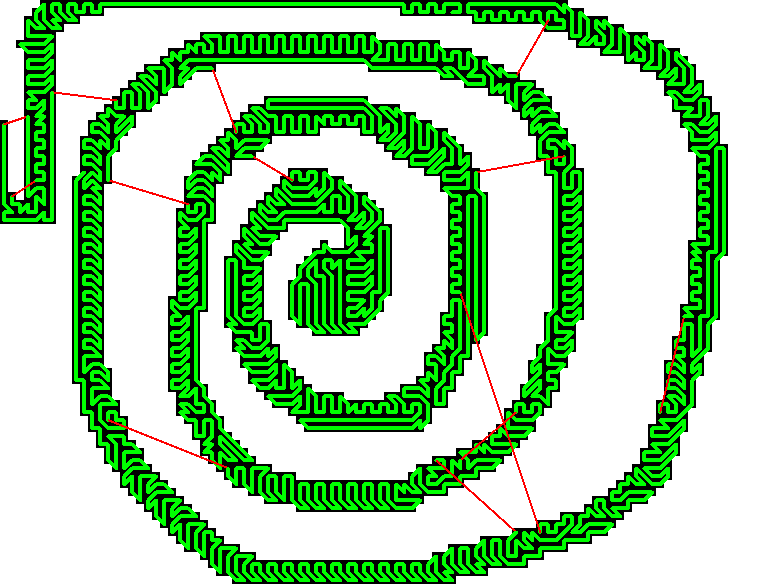
\includegraphics[width=\textwidth]{img/results/sp-4-greedy-harmony.png}
			\multifigcaption
			\caption{Greedy Harmony solution for layer sp-4}
			\label{img:results/sp-4-greedy-harmony}
		\end{minipage}
	\end{center}
\end{figure}

\begin{table}[H]
	\begin{center}
		\begin{tabular}{|m{4cm}||r|r|r|r|}
			\hline

			\multicolumn{3}{|c|}{ 			\cellcolor[gray]{0.7} \textbf{Image}} & \multicolumn{2}{|c|}{sp-4} \\ \hline
			\multicolumn{3}{|c|}{ \cellcolor[gray]{0.7} \textbf{Number of points}} & \multicolumn{2}{|c|}{2448} \\ \hline \hline
			
			\rowcolor{gray!30}
			
			\textbf{Algorithm} & \multicolumn{1}{|c|}{\textbf{Time}} & \multicolumn{1}{|c|}{\textbf{Distance}} & \multicolumn{1}{|c|}{\textbf{Energy}} & \multicolumn{1}{|p{2.5cm}|}{\textbf{Calculation Time $[ms]$}} \\ \hline
				
			Left-to-Right	 & 10913,00 	& 10913,50		& 10985,00 	& 0,26
			 \\ \cline{2-5}
			
			Snake	 & 5574,00		& 5583,19		& 5601,00		& 0,26
			 \\ \cline{2-5}
			
			EF - Time & 2694,00	& 2751,39	& \cellcolor{yellow!80} 2879,00	& 2,46
			  \\ \cline{2-5}
			
			EF - Distance & 2771,00	& 2823,41	& 2944,00 &	19,33
			  \\ \cline{2-5}
			
			EF - Energy & 2789,00 &	2835,24	& 2935,00	& 14,60
			 \\ \cline{2-5}
			
			Greedy &   2547,00	& 2809,71 & 	3194,00	& 663,02
			 \\ \cline{2-5}
			
			Two Opt & 2518,00 &	2705,01	& 2984,00	& 873271,53
			 \\ \cline{2-5}
			
			 Greedy Two Opt & \cellcolor{yellow!80} 2485,00	& \cellcolor{yellow!80} 2703,66	& 3017,00	& 27494,09
			  \\ \cline{2-5}
			
			Harmony Search & 81686,00	& 90773,45	& 115397,00	& 1771093,39
			  \\ \cline{2-5}
			
			Greedy Harmony & 2563,00	& 2811,81	& 3186,00	& 2270588,38
			  \\ \cline{2-5}
			
			Simulated Annealing & 3388,00	& 3745,04	& 4417,00	& 3071234,07
			  \\ \cline{2-5}
			
			Greedy Annealing & 2563,00	& 2802,67	& 3159,00	& 534441,31
			 \\ \hline
			
		\end{tabular}
		\caption{Results for layer sp-4}
		\label{tab:results-sp-4}
	\end{center}
\end{table}



As a second example is chosen a layer with widely spread points. It is presented in figure \ref{img:results/sp-9}. In table \ref{tab:results-sp-9} are presented results. In figures \ref{img:results/sp-9-ef}, \ref{img:results/sp-9-greedy} and \ref{img:results/sp-9-greedy-annealing} are shown example paths.

\begin{figure}[H]
	\begin{center}
		\begin{minipage}{.45\linewidth}
			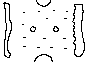
\includegraphics[width=\textwidth]{img/results/sp-9.png}
			\multifigcaption
			\caption{Layer sp-9 \newline}
			\label{img:results/sp-9}
		\end{minipage}
		\hspace{.05\linewidth}
		\begin{minipage}{.45\linewidth}
			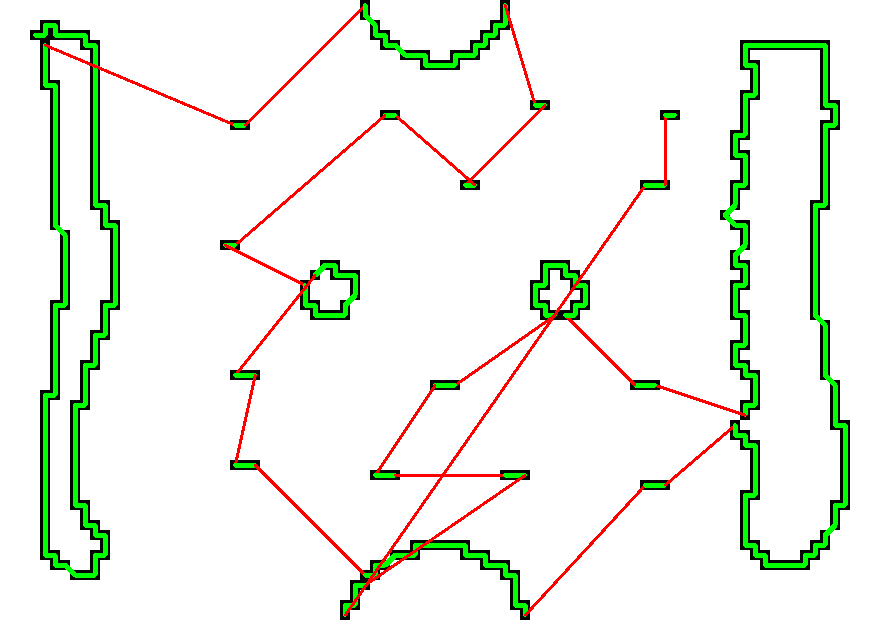
\includegraphics[width=\textwidth]{img/results/sp-9-ef-time.png}
			\multifigcaption
			\caption{Edge Follower solution for layer sp-9 }
			\label{img:results/sp-9-ef}
		\end{minipage}	
		
	\end{center}
\end{figure}

\begin{figure}[H]
	\begin{center}
		\begin{minipage}{.45\linewidth}
			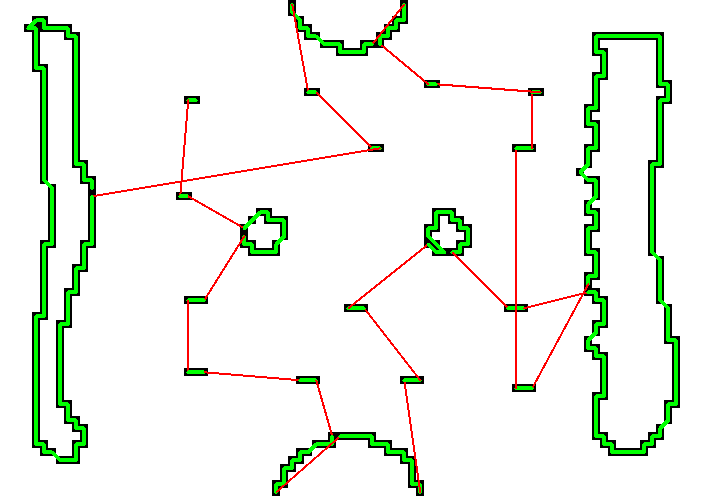
\includegraphics[width=\textwidth]{img/results/sp-9-greedy.png}
			\multifigcaption
			\caption{Greedy solution for layer sp-9 }
			\label{img:results/sp-9-greedy}
		\end{minipage}
		\hspace{.05\linewidth}
		\begin{minipage}{.45\linewidth}
			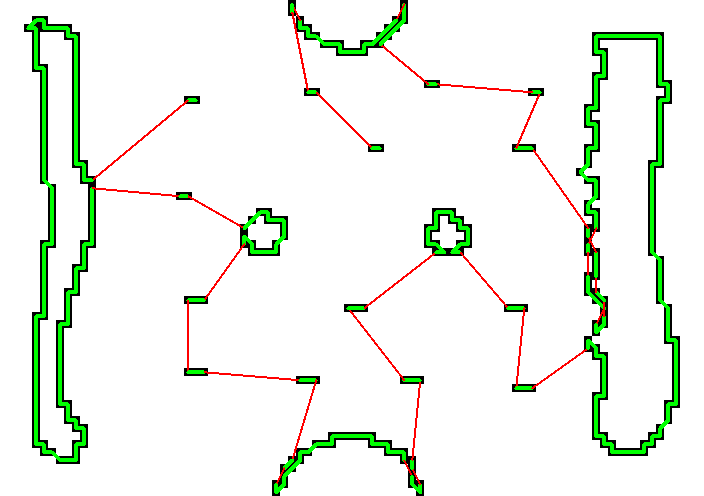
\includegraphics[width=\textwidth]{img/results/sp-9-greedy-annealing.png}
			\multifigcaption
			\caption{Greedy Annealing solution for layer sp-9}
			\label{img:results/sp-9-greedy-annealing}
		\end{minipage}	
		
	\end{center}
\end{figure}

\begin{table}[H]
	\begin{center}
		\begin{tabular}{|m{4cm}||r|r|r|r|}
			\hline
			
			\multicolumn{3}{|c|}{ 			\cellcolor[gray]{0.7} \textbf{Image}} & \multicolumn{2}{|c|}{sp-9} \\ \hline
			\multicolumn{3}{|c|}{ \cellcolor[gray]{0.7} \textbf{Number of points}} & \multicolumn{2}{|c|}{404} \\ \hline \hline
			
			\rowcolor{gray!30}
			
			\textbf{Algorithm} & \multicolumn{1}{|c|}{\textbf{Time}} & \multicolumn{1}{|c|}{\textbf{Distance}} & \multicolumn{1}{|c|}{\textbf{Energy}} & \multicolumn{1}{|p{2.5cm}|}{\textbf{Calculation Time $[ms]$}} \\ \hline
			
			Left-to-Right	 & 8666,00	& 8666,53	& 8727,00	& 0,14
			  \\ \cline{2-5}
			
			Snake & 4448,00	& 4452,43	& 4461,00& 	0,06
			  \\ \cline{2-5}
			
			EF - Time & 625,00	& 683,90& 	796,00&	0,40
			  \\ \cline{2-5}
			
			EF - Distance & 612,00	&  646,02	& 719,00	& 0,64
			  \\ \cline{2-5}
			
			EF - Energy & 640,00	& 666,44	& 739,00	& 0,67
			  \\ \cline{2-5}
			
			Greedy & 621,00	& 651,45	& 718,00	& 24,14
			  \\ \cline{2-5}
			
			Two Opt & 619,00	& 671,69	& 778,00	& 4071,94
			  \\ \cline{2-5}
			
			Greedy Two Opt & 582,00	& 614,54& 	686,00	& 210,73
			  \\ \cline{2-5}
			
			Harmony Search & 12481,00	& 13661,09& 	16949,00	& 75540,56
			  \\ \cline{2-5}
			
			Greedy Harmony & 621,00	& 651,45	& 718,00	& 85273,00
			  \\ \cline{2-5}
			
			Simulated Annealing & 645,00	& 682,56& 	770,00	& 52702,26
			  \\ \cline{2-5}
			
			Greedy Annealing & \cellcolor{yellow!80} 568,00	& \cellcolor{yellow!80}606,87	& \cellcolor{yellow!80}685,00	& 34044,14
			  \\ \hline
			
		\end{tabular}
		\caption{Results for layer sp-9}
		\label{tab:results-sp-9}
	\end{center}
\end{table}

\section{Conclusion}
\begin{figure}
\begin{center}
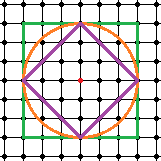
\includegraphics[scale=2]{img/costs}
\end{center}
\caption{Points with cost from red point equal to 3.\\Orange for distance, green for time, and violet for energy}
\label{cost_function_representation}
\end{figure}
As we can see on figure \ref{cost_function_representation}, when algorithm is seeking for closest point, it finds different ones, depending on cost function type. Therefore, if algorithm makes use of this, the results will vary.

Snake algorithm usually provides almost 2 times better results than Left-to-Right, in similar time. For some layers it also provides optimal (or close to it) paths, whereas for other it can give results multiple times worse than optimal.

At least for some algorithms, not only count of points, but also size of whole layer (even if points are only in the middle) can have influence on results or time of calculations, e.g. when algorithm is searching for closest point.

Edge Following algorithm can provide very good results in very short time.

\section{Own contribution}
Michał's contribution:
\begin{itemize}
\item application for tests and graphical representation of results,
\item Left-To-Right algorithm,
\item Snake algorithm,
\item Edge-Following algorithm,
\item layers sp-5 and sp-6,
\item time and energy cost functions,
\item experiments and this report.
\end{itemize}
Piotr's contribution:
\begin{itemize}
\item Greedy algorithm
\item Two Opt algorithm
\item Greedy Two Opt algorithm
\item Harmony Search algorithm
\item Greedy Harmony algorithm
\item Simulated Annealing algorithm
\item Greedy Annealing algorithm
\item layers from sp-7 to sp-10,
\item experiments and this report. 
\end{itemize}

\nocite{*}



\newpage
\bibliographystyle{abbrv}
\bibliography{references}

\end{document}